\documentclass{article}
\usepackage[utf8]{inputenc}
\usepackage[left=3cm, right=3cm, top=2cm]{geometry}
\title{Collisions: Non-linearities without the use of iterative solvers}
\author{Silvin Willemsen}
\date{April 2019}

\usepackage{natbib}
\usepackage{graphicx}
\usepackage{appendix}
\usepackage{amsmath}
\usepackage{amsfonts}
\usepackage{amssymb}

\usepackage{xcolor}
\def\SBcomment[#1]{\textcolor{red}{#1}}
\def\SWcomment[#1]{\textcolor{blue}{#1}}

\begin{document}

\ifpdf % used graphic file format for pdflatex
  \DeclareGraphicsExtensions{.png,.jpg,.pdf,.eps} 
\else  % used graphic file format for latex
  \DeclareGraphicsExtensions{.eps}
\fi

\maketitle

\section{Introduction}
This document shows several examples of non-linearities in physical modelling based on a method recently published by Michele Ducceschi in \cite{Ducceschi2019}.

Energy analysis proves to be a handy tool for verifying whether the devised system is stable or not.

\section{Preamble}
Imagine a mass at location $u = u(t)$ colliding with a barrier at location $b$. Its system would be described as
\begin{equation}\label{eq:massBarrier}
    Mu_{tt} = -K[\eta]_+^\alpha,
\end{equation}
with mass $M$, collision stiffness $K \geq 0$ and non-linearity $\alpha \geq 1$ and $\eta = u - b$ describes the relative displacement between the two colliding bodies.
\begin{equation}
    [\eta]_+ = \frac{\eta + |\eta|}{2}
\end{equation}
describes the positive part of $\eta$ (see Figure \ref{fig:eta}). This can be interpreted as that $\eta$ will only be non-zero when the two colliding bodies are in contact.

\begin{figure}[h]
\centerline{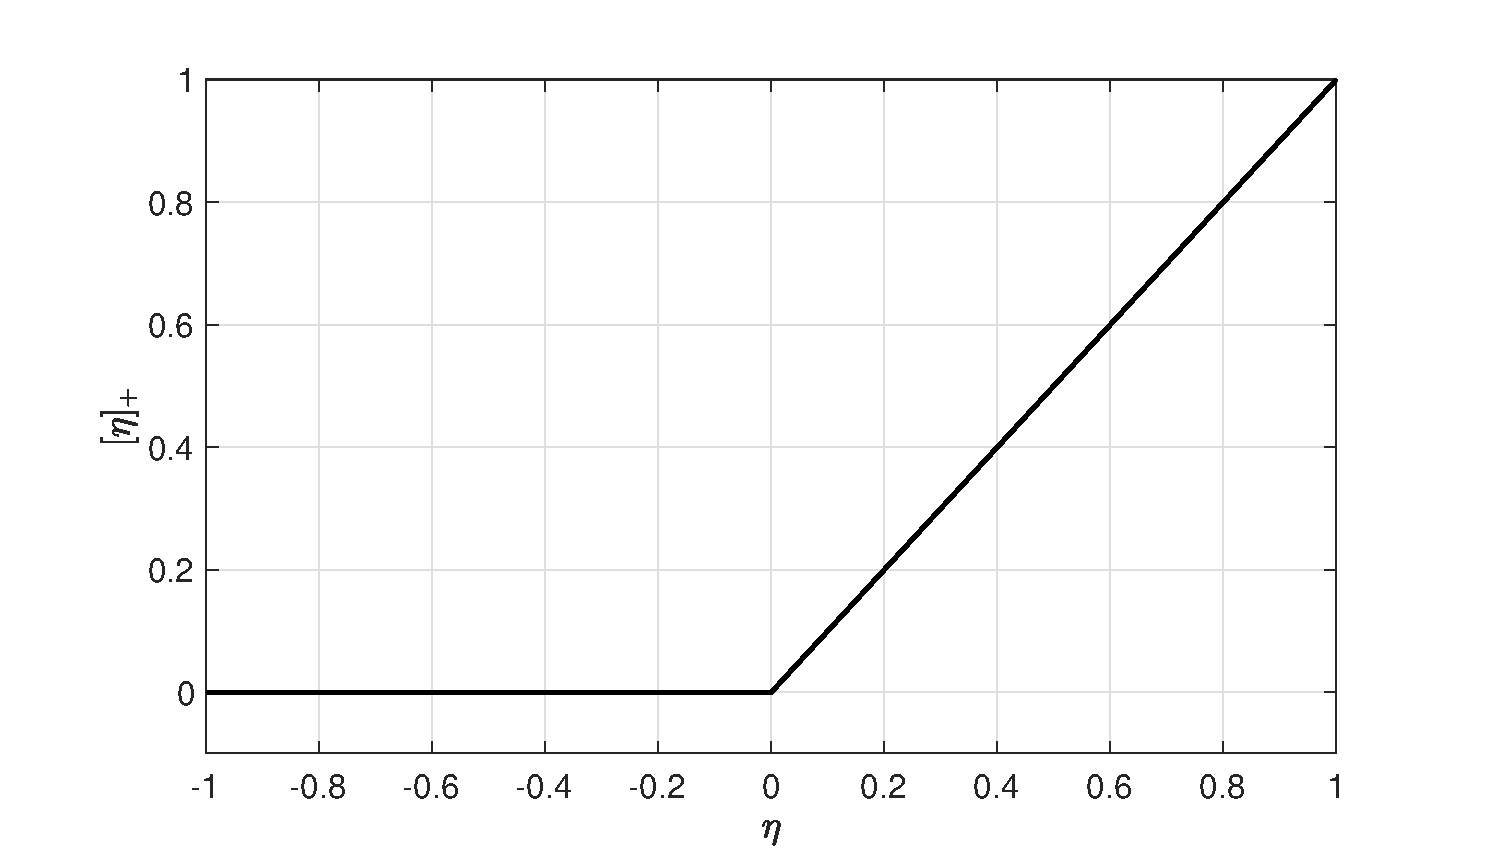
\includegraphics[width=0.6\columnwidth]{eta.eps}}
\caption{\label{fig:eta}{A plot of $[\eta]_+$.}}
\end{figure}

\noindent The second term can be rewritten, to 
\begin{equation}\label{eq:potential}
    \phi'(\eta) = \frac{d\phi}{d\eta}\overset{\text{chain rule}}{\xrightarrow{\hspace*{1.4cm}}}  \frac{\dot{\phi}(\eta)}{\dot{\eta}} =  K[\eta]_+
\end{equation}
yielding
\begin{equation}
    Mu_{tt} = -\phi'(\eta)
\end{equation}
and describes the potential energy of the system. Equation \eqref{eq:potential} is the derivative of
\begin{equation}
    \phi(\eta) = \frac{K}{\alpha+1}[\eta]_+^{\alpha + 1}\ .
\end{equation}
%
According to Ducceschi in \cite{Ducceschi2019}, this potential has been used before in the literature, but when discretised, results in an implicit system for which an iterative solver (such as Newton-Raphson's method) must be employed. In his work, he proposes to rewrite the potential in Eq. \eqref{eq:potential} as
\begin{equation}
    \psi\psi' \quad \text{where} \quad \psi = \sqrt{2\phi} \quad \text{and} \quad \psi' = \frac{\dot{\psi}}{\dot{\eta}}\ .
\end{equation}
\section{Mass - Rigid barrier collision}
The simplest collision case is a point mass colliding with a rigid barrier. If the mass is given a restoring force a simple mass-spring system emerges
\begin{equation}\label{eq:massSpringBarrier}
    Mu_{tt} = -M\omega_0^2u - \psi\psi'
\end{equation}
This system can be written 


where $g^n$ can conveniently be rewritten to:

\begin{equation}
    g = \sqrt{\frac{K(\alpha+1)}{2}}[\eta]_+^{\frac{\alpha-1}{2}}
\end{equation}


\section{Mass - Mass Collision}
The initial idea for this implementation was to make the barrier able to move. However, this would 
Replacing the rigid barrier by a mass


 
\section{Conclusion}
``I always thought something was fundamentally wrong with the universe'' \citep{adams1995hitchhiker}

\bibliographystyle{plain}
\bibliography{references}
\end{document}
